\documentclass[10pt]{beamer}

\usepackage[utf8]{inputenc}
\usepackage{pgfpages}
\usepackage{dirtree}
\setbeamertemplate{note page}[plain]
\setbeameroption{show notes on second screen =left}
\AtEndNote{\vfill \begin{center} mm:hh \end{center}}
\newcommand{\notedir}[1] {
  \note{\dirtree{#1}}}
  \def \ion {$^{\circ}$ }
\usepackage{tcolorbox}
\usepackage{tikz}
\usepackage{tikz-3dplot}
\usetikzlibrary{intersections,calc,,angles,quotes,through}
\usepackage{amsmath}
\usepackage{graphicx}
\usepackage{cases}
\def \heart {\textcolor{blue}{$\heartsuit$} }
\def \C {\mathcal{C}}
\def \orthog {\underline{\perp}}
\def\arcos{\operatorname{arcos}}
\def \deg {^{\circ}}

\newcommand{\vect}[1] {
  \overrightarrow{#1}}

\tcbset{%
	basic/.style={colframe=black,
		      colback=white,
		      top= 0mm,
		      bottom = 2mm,
		      boxsep=0mm
		      }
}
\tikzset{
    invisible/.style={opacity=0},
    visible on/.style={alt={#1{}{invisible}}},
    alt/.code args={<#1>#2#3}{%
      \alt<#1>{\pgfkeysalso{#2}}{\pgfkeysalso{#3}} % \pgfkeysalso doesn't change the path
    },
  }

    
\begin{document}  
    \beamertemplatenavigationsymbolsempty
    \setlength{\abovedisplayskip}{0pt}
    \setlength{\belowdisplayskip}{0pt}
    
    \frame{\frametitle{Droites.}
	 \begin{columns}[t]
	  \column{.5\textwidth}\centering
	  \underline{Equations paramétriques.} \\ \bigskip
	  \begin{figure}[h]
	   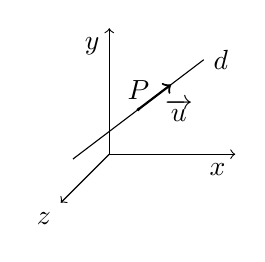
\begin{tikzpicture}[scale=0.4]
					%\draw[help lines] (-3,-3) grid (3,3); 				
					%AXES
					\draw[->] (0,0,0) -- (4,0,0) coordinate[label=below left:$x$]();
					\draw[->] (0,0,0) -- (0,4,0) coordinate[label=below left:$y$]();
					\draw[->] (0,0,0) -- (0,0,4) coordinate[label=below left:$z$]();
					\draw (0,1,3) --coordinate[label=above:$P$](P) (3,3,0)node[right]{$d$};
					\fill (P) circle (0.06);
					\draw[->,thick] (P) --coordinate[label=below right :$\vect{u}$,yshift=1mm](u) +($0.5*(3,3,0)-0.5*(P)$);
	  \end{tikzpicture}
	  \end{figure}
	  \begin{align*}
	   d \equiv&\ P + \lambda \vect{u}, \quad (\lambda \in \mathbb{R}) \\
	     \equiv& \begin{cases}
	              x = P_x + \lambda u_x, \\
	              y = P_y + \lambda u_y, \\
	              z = P_z + \lambda u_z. \\
	             \end{cases} 
	  \end{align*} 
	  \medskip
	  
	  On fait varier le paramètre, on a les points de la droite. \\ \medskip
	  Sans les termes indépendants, on a les vecteurs directeurs de la droite.
	  \column{.5\textwidth}\centering
	  \underline{Equations cartésiennes.} \\ \bigskip
	  \begin{figure}[h]
	   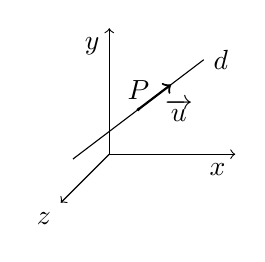
\begin{tikzpicture}[scale=0.4]
					%\draw[help lines] (-3,-3) grid (3,3); 				
					%AXES
					\draw[->] (0,0,0) -- (4,0,0) coordinate[label=below left:$x$]();
					\draw[->] (0,0,0) -- (0,4,0) coordinate[label=below left:$y$]();
					\draw[->] (0,0,0) -- (0,0,4) coordinate[label=below left:$z$]();
					\draw (0,1,3) --coordinate[label=above:$P$](P) (3,3,0)node[right]{$d$};
					\fill (P) circle (0.06);
					\draw[->,thick] (P) --coordinate[label=below right :$\vect{u}$,yshift=1mm](u) +($0.5*(3,3,0)-0.5*(P)$);
	  \end{tikzpicture}
	  \end{figure}
	  $$ d \equiv \frac{x-P_x}{u_x}=\frac{y-P_y}{u_y}=\frac{z-P_z}{u_z}.$$ 
	  \vspace{3.7em}
	  
	  Un point appartient à la droite si ses coordonnées vérifient l'équation. \\ \medskip
	  Un vecteur est $\parallel$ à la droite s'il vérifie l'équation sans termes indép.
	  
	 \end{columns}
\notedir{%
.1 Représenter les droites par des équations.
.2 Droite définie par point et direction (vecteur)..
.3 Equations paramétriques.
.4 En variant paramètre, on obtient les points..
.4 En variant paramètre, sans termes indépendants, on obtient vecteurs directeurs..
.3 Equations cartésiennes.
.4 Point appartient à droite s'il vérifie équations..
.4 Vecteur parallèle à droite s'il vérifie équations sans termes indépendants..
}
    }

    \frame{ \frametitle{Droites.}
	    \begin{columns}[t]
	     \column{.333\textwidth}\centering
	     \underline{Parallèles.}
	     \begin{figure}[h]
	   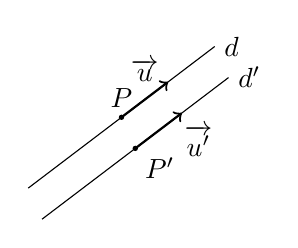
\begin{tikzpicture}[scale=0.57]
					%\draw[help lines] (-3,-3) grid (3,3); 				
					%AXES
					%\draw[->] (0,0,0) -- (4,0,0) coordinate[label=below left:$x$]();
					%\draw[->] (0,0,0) -- (0,4,0) coordinate[label=below left:$y$]();
					%\draw[->] (0,0,0) -- (0,0,4) coordinate[label=below left:$z$]();
					\draw (0,1,3) --coordinate[label=above:$P$](P) (3,3,0)node[right]{$d$};
					\draw (0.5,0.5,3.5) --coordinate[label=below right:$P'$](P') (3.5,2.5,0.5)node[right]{$d'$};
					\fill (P) circle (0.06);
					\fill (P') circle (0.06);
					\draw[->,thick] (P) --coordinate[label=above :$\vect{u}$,yshift=1mm](u) +($0.5*(3,3,0)-0.5*(P)$);
					\draw[->,thick] (P') --coordinate[label=below right :$\vect{u'}$,yshift=2mm,xshift=2mm](u') +($0.5*(3.5,2.5,0.5)-0.5*(P')$);
	  \end{tikzpicture}
	  \end{figure} \bigskip \flushleft
	  \textit{Parallèles} : vecteurs directeurs multiples l'un de l'autre. \\ \medskip
	  \textit{Confondues} : parallèles et point en commun.
	     \column{.333\textwidth}\centering
	     \underline{Sécantes.}
	     \begin{figure}[h]
	   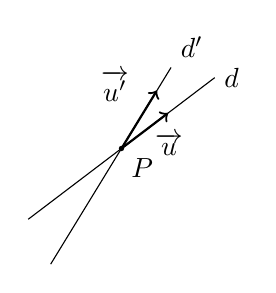
\begin{tikzpicture}[scale=0.57]
					%\draw[help lines] (-3,-3) grid (3,3); 				
					%AXES
					%\draw[->] (0,0,0) -- (4,0,0) coordinate[label=below left:$x$]();
					%\draw[->] (0,0,0) -- (0,4,0) coordinate[label=below left:$y$]();
					%\draw[->] (0,0,0) -- (0,0,4) coordinate[label=below left:$z$]();
					\draw (0,1,3) --coordinate[label=below right:$P$](P) (3,3,0)node[right]{$d$};
					\fill (P) circle (0.06);
					\draw (0.5,0,3) -- (P) -- +($.7*(P)-.7*(0.5,0,3)$)node[above right]{$d'$};
					\draw[->,thick] (P) --coordinate[label=below right :$\vect{u}$,yshift=1mm](u) +($0.5*(3,3,0)-0.5*(P)$);
					\draw[->,thick] (P) --coordinate[label=above left :$\vect{u'}$,yshift=1mm](u) +($.5*(P)-.5*(0.5,0,3)$);
	  \end{tikzpicture}
	  \end{figure}\flushleft\vspace{2mm}
	  
	  \textit{Sécantes} : Solution du système formé par les équations cartésiennes des droites est un point.
	     \column{.37\textwidth}\centering
	     \underline{Gauches.}
	     \begin{figure}[h]
	   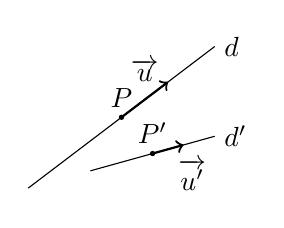
\begin{tikzpicture}[scale=0.57]
					%\draw[help lines] (-3,-3) grid (3,3); 				
					%AXES
					%\draw[->] (0,0,0) -- (4,0,0) coordinate[label=below left:$x$]();
					%\draw[->] (0,0,0) -- (0,4,0) coordinate[label=below left:$y$]();
					%\draw[->] (0,0,0) -- (0,0,4) coordinate[label=below left:$z$]();
					\draw (0,1,3) --coordinate[label=above:$P$](P) (3,3,0)node[right]{$d$};
					\draw (1,1,2) --coordinate[label=above:$P'$](P') (3,1,0)node[right]{$d'$};
					\fill (P) circle (0.06);
					\fill (P') circle (0.06);
					\draw[->,thick] (P) --coordinate[label=above :$\vect{u}$,yshift=1mm](u) +($0.5*(3,3,0)-0.5*(P)$);
					\draw[->,thick] (P') --coordinate[label=below right :$\vect{u'}$](u') +($0.5*(3,1,0)-0.5*(P')$);
	  \end{tikzpicture}
	  \end{figure}\flushleft
	  \vspace{10mm}
	  \textit{Gauches} : Ni parallèles ni sécantes. \\ \medskip
	  \textit{Orthogonales} : Gauches et directions perpendiculaires.
	    \end{columns}
\notedir{%
.1 Positions des droites..
.2 Parallèles..
.3 vecteurs multiples l'un de l'autre..
.4 Confondues si point en commun..
.2 Sécantes..
.3 Système pour trouver intersect\ion et solution est un point..
.2 Gauches..
.3 Vecteurs non multiples l'un de l'autre et pas\\ \hspace{5mm} d'intersect\ion..
.4 Orthogonales si vecteurs perpendiculaires..
}
	  }
	
    \frame{ \frametitle{Plans.}
    \begin{columns}[t]
	  \column{.5\textwidth}\centering
	  \underline{Equations paramétriques.} \\ \bigskip
	  \begin{figure}[h]
	   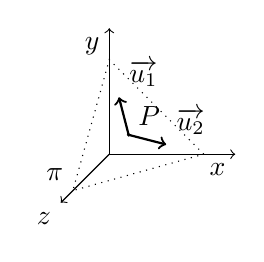
\begin{tikzpicture}[scale=0.4]
					%\draw[help lines] (-3,-3) grid (3,3); 				
					%AXES
					\draw[->] (0,0,0) -- (4,0,0) coordinate[label=below left:$x$]();
					\draw[->] (0,0,0) -- (0,4,0) coordinate[label=below left:$y$]();
					\draw[->] (0,0,0) -- (0,0,4) coordinate[label=below left:$z$]();
					\draw[dotted] (3,0,0) -- (0,3,0) -- (0,0,3)node[above left]{$\pi$} -- cycle;
					\coordinate[label=above right:$P$](P) at (1,1,1);
					\fill (P) circle (0.06);
					\draw[->,thick] (P) -- +($0.5*(0,3,0)-0.5*(P)$) coordinate[label= above right :$\vect{u_1}$](u_1);
					\draw[->,thick] (P) -- +($0.5*(3,0,0)-0.5*(P)$) coordinate[label=above right:$\vect{u_2}$](u_2);
	  \end{tikzpicture}
	  \end{figure}
	  \begin{align*}
	   \pi \equiv&\ P + \lambda \vect{u_1} + \mu \vect{u_2} , \quad (\lambda,\mu \in \mathbb{R}) \\
	     \equiv& \begin{cases}
	              x = P_x + \lambda u_{1_x} + \mu u_{2_x}, \\
	              y = P_y + \lambda u_{1_y} + \mu u_{2_y}, \\
	              z = P_z + \lambda u_{1_z} + \mu u_{2_z}. \\
	             \end{cases} 
	  \end{align*} 
	  \medskip
	  
	  On fait varier les paramètres, on obtient les points du plan. \\ \medskip
	  Sans les termes indépendants, on a les vecteurs directeurs du plan.
	  \column{.5\textwidth}\centering
	  \underline{Equations cartésiennes.} \\ \bigskip
	  \begin{figure}[h]
	   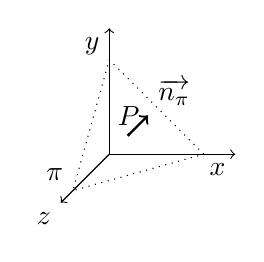
\begin{tikzpicture}[scale=0.4]
					%\draw[help lines] (-3,-3) grid (3,3); 				
					%AXES
					\draw[->] (0,0,0) -- (4,0,0) coordinate[label=below left:$x$]();
					\draw[->] (0,0,0) -- (0,4,0) coordinate[label=below left:$y$]();
					\draw[->] (0,0,0) -- (0,0,4) coordinate[label=below left:$z$]();
					\draw[dotted] (3,0,0) -- (0,3,0) -- (0,0,3)node[above left]{$\pi$} -- cycle;
					\coordinate[label=above:$P$](P) at (1,1,1);
					\fill (P) circle (0.06);
					\draw[->,thick] (P) -- +(1,1,1) coordinate[label= above right :$\vect{n_{\pi}}$](n_pi);
	  \end{tikzpicture}
	  \end{figure}
	  $$ \pi \equiv n_{\pi_x}x + n_{\pi_y}y + n_{\pi_z}z +d = 0.$$ 
	  \vspace{4em}
	  
	  Un point appartient au plan si ses coordonnées vérifient l'équation. \\ \medskip
	  Un vecteur est $\parallel$ au plan s'il vérifie l'équation sans termes indép.
	 \end{columns}
	 
	 \notedir{%
.1 Représenter les plans par des équations.
.2 Plan défini par point et 2 directions (vecteurs)..
.3 Equations paramétriques.
.4 En variant paramètres, on obtient les points..
.4 En variant paramètres, sans termes indépendants, on obtient vecteurs directeurs..
.3 Equations cartésiennes.
.4 Formée avec vecteur perpendiculaire au plan..
.4 Point appartient au plan s'il vérifie équation..
.4 Vecteur parallèle au plan s'il vérifie équations sans termes indépendants..
}
    }
	
	\frame{ \frametitle{Plans.}
	    \begin{columns}[t]
	     \column{.5\textwidth}\centering
	     \underline{Parallèles.}
	     \begin{figure}[h]
	   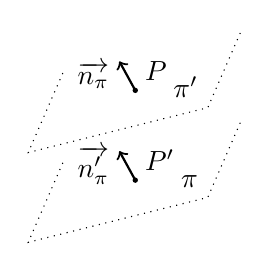
\begin{tikzpicture}[scale=0.57]
					%\draw[help lines] (-3,-3) grid (3,3); 				
					%AXES
					%\draw[->] (0,0,0) -- (4,0,0) coordinate[label=below left:$x$]();
					%\draw[->] (0,0,0) -- (0,4,0) coordinate[label=below left:$y$]();
					%\draw[->] (0,0,0) -- (0,0,4) coordinate[label=below left:$z$]();
					\draw[dotted] (0,3,-2) -- (0,2,0) -- (4,3,0)node[above left]{$\pi '$} -- +(0,1,-2);
					\draw[dotted] (0,1,-2) -- (0,0,0) -- (4,1,0)node[above left]{$\pi$} --+(0,1,-2) ;
					\coordinate[label=above right:$P$](P) at (2,3,-1);
					\coordinate[label=above right:$P'$](P') at (2,1,-1);
					\fill (P) circle (0.06);
					\fill (P') circle (0.06);
					\draw[->,thick] (P) --coordinate[label=left :$\vect{n_{\pi}}$,xshift=-1mm]() +($.2*(-1,4,2)$);
					\draw[->,thick] (P') --coordinate[label=left :$\vect{n_{\pi}'}$,xshift=-1mm]() +($.2*(-1,4,2)$);
	  \end{tikzpicture}
	  \end{figure} \bigskip \flushleft
	  \textit{Parallèles} : vecteurs normaux multiples l'un de l'autre. \\ \medskip
	  \textit{Confondus} : parallèles et point en commun.
	     \column{.5\textwidth}\centering
	     \underline{Sécants.}
	     \begin{figure}[h]
	   \begin{tikzpicture}[scale=0.57]
					%\draw[help lines] (-3,-3) grid (3,3); 				
					%AXES
					
			          %projection ($(X)!(B')!(B)$)
			          %nommer chemin 'name path
			          %intersection \path [name intersections={of=d and gb,by=G}];
			         
			          \draw  (0,0,0)  node[below] {$d$} -- (0,2,-1);
			          
			          
			          
			          \draw[dotted] (-2,-0.5,0) -- +(0,2,-1) -- (2,2.5,-1) node[above left]{$\pi$} -- +(0,-2,1) -- cycle;
			          \draw[dotted] (0,2,2)  -- +(0,-2,1) node[below]{$\pi '$} -- (0,0,-1) -- +(0,2,-1) -- cycle;
			          
				  
	  \end{tikzpicture}
	  \end{figure}\flushleft\vspace{8mm}
	  
	  \textit{Sécantes} : Solution du système formé par les équations cartésiennes des plans est une droite.
	    \end{columns}
\notedir{%
.1 Positions des plans..
.2 Parallèles..
.3 vecteurs normaux multiples l'un de l'autre..
.4 Confondus si point en commun..
.2 Sécants..
.3 Système pour trouver intersect\ion et solution est une droite..
}
	  }
	  
	  \frame{ \frametitle{Droites et Plans.}
	    \begin{columns}[t]
	     \column{.5\textwidth}\centering
	     \underline{Parallèles.}
	     \begin{figure}[h]
	   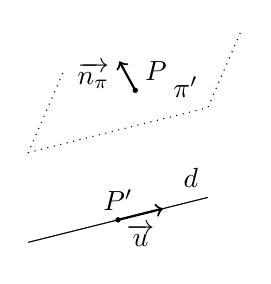
\begin{tikzpicture}[scale=0.57]
					%\draw[help lines] (-3,-3) grid (3,3); 				
					%AXES
					%\draw[->] (0,0,0) -- (4,0,0) coordinate[label=below left:$x$]();
					%\draw[->] (0,0,0) -- (0,4,0) coordinate[label=below left:$y$]();
					%\draw[->] (0,0,0) -- (0,0,4) coordinate[label=below left:$z$]();
					\draw[dotted] (0,3,-2) -- (0,2,0) -- (4,3,0)node[above left]{$\pi '$} -- +(0,1,-2);
					\draw  (0,0,0) -- (4,1,0)node[above left]{$d$} ;
					\coordinate[label=above right:$P$](P) at (2,3,-1);
					\coordinate[label=above:$P'$](P') at (2,0.5,0);
					\fill (P) circle (0.06);
					\fill (P') circle (0.06);
					\draw[->,thick] (P) --coordinate[label=left :$\vect{n_{\pi}}$,xshift=-1mm]() +($.2*(-1,4,2)$);
					\draw[->,thick] (P') --coordinate[label=below :$\vect{u}$]() +($.5*(4,1,0)-.5*(P')$);
	  \end{tikzpicture}
	  \end{figure} \bigskip \flushleft
	  \textit{Parallèles} : vecteur de la droite vérifie équation cartésienne du plan sans termes indep. \\ \medskip
	  \textit{Confondus} : parallèles et point en commun.
	     \column{.5\textwidth}\centering
	     \underline{Sécants.}
	     \begin{figure}[h]
	   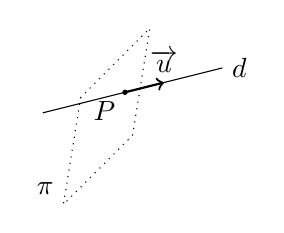
\begin{tikzpicture}[scale=0.57]
					%\draw[help lines] (-3,-3) grid (3,3); 				
					%AXES
					
			          %projection ($(X)!(B')!(B)$)
			          %nommer chemin 'name path
			          %intersection \path [name intersections={of=d and gb,by=G}];
			         
			          \path[name path=d_i]  (0,0,0) -- (0,2,-1);			          
			          \draw[name path=d] (-2,0.5,-1) -- (2,1.5,-1)node[right]{$d$};
			          \path [name intersections={of=d and d_i,by=P}];
			          \coordinate[label=below left:$P$]() at (P);
			          \fill (P) circle (0.06);
			          \draw[dotted] (0,2,2) -- +(0,-2,1) node[above left]{$\pi$} -- (0,0,-1) -- +(0,2,-1) -- cycle;
			          \draw[->,thick] (P) -- +($.4*(2,1.5,-1)-.4*(P)$) node[above]{$\vect{u}$};
			          %\draw[->,thick] (P) -- +(1,0,0)node[below]{$n_{\pi}$};
				  
	  \end{tikzpicture}
	  \end{figure}\flushleft\vspace{14mm}
	  
	  \textit{Sécantes} : vecteur de la droite ne vérifie pas équation cartésienne du plan sans termes indep.
	    \end{columns}
\notedir{%
.1 Positions des droites et plans..
.2 Parallèles..
.3 Vecteur directeur de droite vérifie équation cartésienne\\ \hspace{5mm} plan sans terme indépendant..
.4 Confondus si point en commun..
.2 Sécants..
.3 Vecteur directeur de droite ne vérifie pas équation cartésienne plan sans terme indépendant..
}
	  }
	  
	  \frame{\frametitle{Distances.}
	  \begin{columns}[c]
	   \column{.3\textwidth}\centering
	   
	  \begin{figure}[h]
	   \begin{tikzpicture}[scale=0.38]
					%\draw[help lines] (-3,-3) grid (3,3); 				
					%AXES
					\draw[->] (0,0,0) -- (4,0,0) coordinate[label=below left:$x$]();
					\draw[->] (0,0,0) -- (0,4,0) coordinate[label=below left:$y$]();
					\draw[->] (0,0,0) -- (0,0,4) coordinate[label=below left:$z$]();
					\coordinate[label=above:$A$](A) at (1,1,1);
					\coordinate[label=above:$B$](B) at (2,2,1);
					\fill (A) circle (0.06);
					\fill (B) circle (0.06);					
	  \end{tikzpicture}
	  \end{figure} 
	  \column{.8\textwidth}\centering
	  $\mathcal{D}(A,B) = \sqrt{(A_x-B_x)^2+(A_y-B_y)^2+(A_z-B_z)^2}$.
	  \end{columns}
	  \begin{columns}[c]
	   \column{.3\textwidth}\centering
	   
	  \begin{figure}[h]
	   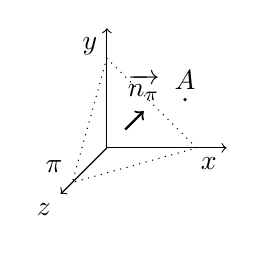
\begin{tikzpicture}[scale=0.38]
					%\draw[help lines] (-3,-3) grid (3,3); 				
					%AXES
					\draw[->] (0,0,0) -- (4,0,0) coordinate[label=below left:$x$]();
					\draw[->] (0,0,0) -- (0,4,0) coordinate[label=below left:$y$]();
					\draw[->] (0,0,0) -- (0,0,4) coordinate[label=below left:$z$]();
					\coordinate[label=above:$A$](A) at (3,2,1);
					\fill (A) circle (0.06);
					\draw[dotted] (3,0,0) -- (0,3,0) -- (0,0,3)node[above left]{$\pi$} -- cycle;	
					\draw[->,thick] (1,1,1) -- +(1,1,1) coordinate[label= above :$\vect{n_{\pi}}$](n_pi);
	  \end{tikzpicture}
	  \end{figure} 
	  \column{.8\textwidth}\centering
	  $\mathcal{D}(A,\pi) = \dfrac{|n_{\pi_x}A_x + n_{\pi_y}A_y + n_{\pi_z}A_z + d|}{|\vect{n_{\pi}}|}$.
	  \end{columns}
	  \begin{columns}[c]
	   \column{.3\textwidth}\centering
	   
	  \begin{figure}[h]
	   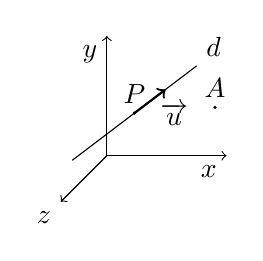
\begin{tikzpicture}[scale=0.38]
					%\draw[help lines] (-3,-3) grid (3,3); 				
					%AXES
					\draw[->] (0,0,0) -- (4,0,0) coordinate[label=below left:$x$]();
					\draw[->] (0,0,0) -- (0,4,0) coordinate[label=below left:$y$]();
					\draw[->] (0,0,0) -- (0,0,4) coordinate[label=below left:$z$]();
					\coordinate[label=above:$A$](A) at (4,2,1);
					\fill (A) circle (0.06);
					\draw (0,1,3) --coordinate[label=above:$P$](P) (3,3,0)node[ above right]{$d$};
					\fill (P) circle (0.06);
					\draw[->,thick] (P) --coordinate[label=below right :$\vect{u}$,yshift=1mm](u) +($0.5*(3,3,0)-0.5*(P)$);
	  \end{tikzpicture}
	  \end{figure} 
	  \column{.8\textwidth}\centering
	  $\mathcal{D}(A,d) = \dfrac{|\vect{AP}\wedge\vect{u}|}{|\vect{u}|}$.
	  \end{columns}
\notedir{%
.1 Distances..
.2 Point - Point..
.3 Point - Plan..
.4 Valeur absolue de l'équation cartésienne du plan en remplaçant x,y,z par coordonnées du point divisé par longueur du vecteur normal utilisé dans équation du plan..
.4 Si oubli, calculer distance entre le point et sa projection sur le plan..
.3 Point - Droite..
.4 Valeur absolue de produit vectoriel de $\vect{AP}$ et $\vect{u}$ divisé par longueur de $\vect{u}$ ($P$ point quelconque appartenant à la droite)..
.4 Si oubli, calculer distance entre le point et sa projection sur la droite..
}
	  }
  
\end{document}

%%% Local Variables:
%%% mode: latex
%%% TeX-master: t
%%% End:
